%% NEW TEMPLATE!!
% !TEX root = DesignDocument.tex


\chapter{Overview and concept of operations}

%%The overview should take the form of an executive summary.  Give the reader a feel 
%%for the purpose of the document, what is contained in the document, and an idea 
%%of the purpose for the system or product. 

\section{Team Members and Team Name}
Team: ARM Cluster: A Research Tool.\\
Team members: Andrew Hoover Christine Sorensen

\section{Client}
%%A description of the client or customer.

The client is Dr. Christer Karlsson, an associate professor at the South Dakota School of Mines and Technology.

\section{Project}
%%A high level description of the project.

This project is a research project with the goal of creating the most effecient cluster of single board computers possible within a budget of \$1,200. This will include choosing which single board computer to use, determining how many can be purchased without going over budget keeping in mind any other costs, and assembling the cluster. It will also include benchmarking the cluster accross as many different communication protocols and topologies as possible. 

\subsection{Purpose of the System}
%%What is the purpose of the system or product? 

The end goal is to learn about networking, parallelization, and different communication methods. Once as much information is gathered as possible, the resulting cluster and configuration will be returned to Dr. Karlsson for him to decide what to use the project for in the future. Possibilities include handing it off to other students for continuing work, or other research.


\section{Deliverables}

%%Provide a complete description of the client requested deliverables.   This section should be the section your software contract references.   
\begin{itemize}
	\item ARM Cluster
	\item Research Symposium
	\item Design Fair
	\item Documentation
\end{itemize}

\section{System Description}

The system will contain several pieces of hardware, and a benchmarking tool. 

\subsection{Major System Component \#1}
%%Describe briefly the role this major component plays in this system. 

The first and most evident component to the cluster is the physical hardware that will go in to building it. This includes several items. There will be an unmanaged switch to allow for Ethernet connection between the devices, Cat 5 Ethernet cables to take advantage of the 1 Gigabit Ethernet ports availible in modern single board computers, a power supply, and a piece of acrylic board to attach everything to. 

\subsection{Major System Component \#2}
%%Describe briefly the role this major component plays in this system. 

Another important component is a way to test the speed of the cluster. This is essential to learn which method of clustering the devices is most effecient. As such we will dedicate a substancial amount of time to finding a reliable and useful benchmarking tool that is an industry standard so that we can compare our cluster to other similar projects.

\subsection{Major System Component \#3}
%%Describe briefly the role this major component plays in this system. 

\section{Systems Goals}
%%Briefly describe the overall goals this system plans to achieve.
%%These goals are typically provided by the stakeholders.  This is not
%%intended to be a detailed requirements listing.  Keep in mind that
%%this section is still part of the Overview.

\begin{itemize}
	\item Create a cluster of 6 - 12 single board computers.
	\item Create the fastest and most effecient in terms of cost and operation cluster possible.
	\item Have all computers, power supply, switch, memory, cables and power strips needed to be at or below \$1,200.
	\item Know which computer is the fastest in terms of Gigaflops per dollar per watt.
	\item Use other communication modes than Ethernet.
	\item Benchmark the new communications.
\end{itemize}

\section{System Overview and Diagram}
%%Provide a more detailed description of the major system components
%%without getting too detailed.  This section should contain a
%%high-level block and/or flow diagram of the system highlighting the
%%major components.  See Figure~\ref{systemdiagram}.  This is a floating
%%figure environment.  \LaTeX\ will try to put it close to where it was
%%typeset but will not allow the figure to be split if moving it can not
%%happen.  Figures, tables, algorithms and many other floating
%%environments are automatically numbered and placed in the appropriate
%%type of table of contents.  You can move these and the numbers will
%%update correctly.

The systems components were used to achieve the goals in specific ways. First the cluster was desgined in a Star Topology, as described in Figure~\ref{star}. This was accomplished with the hardware purchased for the cluster.

%% SAMPLE IMAGE WITH STUFF
\begin{figure}[tbh]
\begin{center}
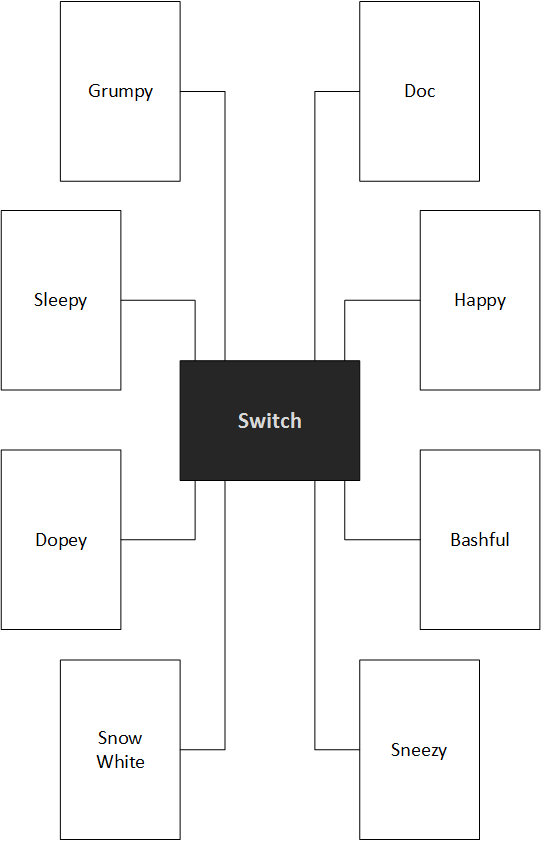
\includegraphics[width=0.75\textwidth]{cluster_star.png}
\end{center}
\caption{Star Topology. \label{star}}
\end{figure}

\section{Technologies Overview}
%%This section should contain a list of specific technologies used to
%%develop the system.  The list should contain the name of the
%%technology, brief description, link to reference material for further
%%understanding, and briefly how/where/why it was used in the system.
%%See Table~\ref{somenumbers}.  This is a floating table environment.
%%\LaTeX\ will try to put it close to where it was typeset but will not
%%allow the table to be split.

Many different technologies were used in the completion of this project. First, several programming languages were used, as described in Table~\ref{languages}. Also, the open source project High Performance LINPACK was used to benchmark the cluster. ATLAS, Automatically Tuned Linear Algebra Software, and MPI, Message Passing Interface, were used to build LINPACK, ATLAS for the linear algebra libraries to perform the benchmarking computations and MPI to run the tests in parallel accross the cluster.

%%SAMPLE TABLE WITH SHIT AND STUFF
\begin{table}[tbh]
\caption{Programming languages and uses. \label{languages}}
\begin{center}
\begin{tabular}{|r|l|}
  \hline
  Python & Create scripting tools to configure the cluster. \\
  Bash &  \\ \cline{1-2}
  C & Test MPI code, GPIO communication. \\ \cline{1-2}
  C++ & Benchmark individual devices. \\
  \hline
\end{tabular}
\end{center}
\end{table}

